%%%%%%%%%%%%%%%%%%%%%%%%%%%%%%%%%%%%%%%%%%%%%%%%%
%%%%%%%%%%%%%%%%%%%%%%%%%%%%%%%%%%%%%%%%%%%%%%%%%
%%%      IGNORE THIS FIRST PART        %%%%%%%%%%   EXCEPT TO ENTER/DELETE YOUR NAME WHERE INDICATED
%%%%%%%%%%%%%%%%%%%%%%%%%%%%%%%%%%%%%%%%%%%%%%%%%
%%%%%%%%%%%%%%%%%%%%%%%%%%%%%%%%%%%%%%%%%%%%%%%%%

\documentclass[12pt]{amsart}
\usepackage{amsmath, amssymb, amsthm}
\usepackage{mathrsfs}
\usepackage{array}
\usepackage{enumitem}
\usepackage[usenames,dvipsnames]{xcolor}
\usepackage{graphicx}
\usepackage{fancyhdr}
\usepackage{caption}
\usepackage{hyperref}
\usepackage[labelformat=simple]{subcaption}
\usepackage[framemethod=default]{mdframed}
\usepackage{framed}
\usepackage{setspace}
\usepackage{changepage}
\usepackage{graphicx}   

\newmdenv[linecolor=NavyBlue,backgroundcolor=White]{myframe}
\renewcommand\thesubfigure{(\Alph{subfigure})}
\renewcommand\thesubfigure{(\Alph{subfigure})}

\newcounter{problem_number}[section]
\newcommand{\num}{\refstepcounter{problem_number}\arabic{problem_number}}
\newcommand{\numlabel}[1]{\refstepcounter{problem_number}\label{#1}\arabic{problem_number}}

\newtheorem*{theorem}{Theorem}
\newtheoremstyle{named}{}{}{\itshape}{}{\bfseries}{.}{.5em}{\thmnote{#3}}
\theoremstyle{named}
\newtheorem*{namedtheorem}{Theorem}

\newenvironment{prf}
{\medskip\begin{color}{Gray}\begin{framed}\begin{color}{NavyBlue}\begin{proof}[Proof]
\doublespacing}
{\end{proof}\end{color}\end{framed}\end{color}\medskip}

\newenvironment{soln}
{\begin{color}{Gray}\begin{framed}\begin{color}{NavyBlue}\begin{proof}[Solution]
\doublespacing}
{\end{proof}\end{color}\end{framed}\end{color}}

\theoremstyle{definition}
\newtheorem{problem}{Problem}

\setenumerate[1]{label=(\roman*)}

\newcommand{\jeff}[1]{\textbf{\textcolor{WildStrawberry}{#1}}}
\newcommand{\student}[1]{\textbf{\textcolor{Orange}{#1}}}
\newcommand{\peer}[1]{\textbf{\textcolor{ForestGreen}{#1}}}

\textwidth=6.5in
\hoffset-.75in
\textheight=9in
\voffset-.75in
\footskip=30pt
\headheight=14pt
\pagestyle{fancy}
\lhead{\emph{\textcolor{Gray}{Chapter 1 Bonus Homework}}}			%%  UPDATE THE VERSION HERE!!!
\rhead{\emph{\textcolor{Gray}{student-name}}}			%%  ENTER/DELETE YOUR NAME HERE!!!
\chead{\emph{\textcolor{Gray}{MATH 309}}}
\cfoot{\thepage}
\renewcommand{\headrulewidth}{0.35pt}
\renewcommand{\footrulewidth}{0.35pt}
\thispagestyle{fancy}

%%%%%%%%%%%%%%%%%%%%%%%%%%%%%%%%%%%%%%%%%%%%%%%%%
%%%%%%%%%%%%%%%%%%%%%%%%%%%%%%%%%%%%%%%%%%%%%%%%%
%%%       ADD CUSTOM COMMANDS HERE     %%%%%%%%%%
%%%%%%%%%%%%%%%%%%%%%%%%%%%%%%%%%%%%%%%%%%%%%%%%%
%%%%%%%%%%%%%%%%%%%%%%%%%%%%%%%%%%%%%%%%%%%%%%%%%

\newcommand{\F}{\mathbb F}
\newcommand{\N}{\mathbb N}
\newcommand{\Q}{\mathbb Q}
\newcommand{\R}{\mathbb R}
\renewcommand{\S}{\mathbb S}
\newcommand{\Z}{\mathbb Z}
\newcommand{\RP}{\mathbb{RP}}

\newcommand{\Ff}{\mathcal F}
\newcommand{\Ll}{\mathcal L}
\newcommand{\Pp}{\mathcal P}
\newcommand{\Rr}{\mathcal R}

\newcommand{\Line}[1]{\overleftrightarrow{#1}}
\newcommand{\Ray}[1]{\overrightarrow{#1}}

%%%%%%%%%%%%%%%%%%%%%%%%%%%%%%%%%%%%%%%%%%%%%%%%%
%%%%%%%%%%%%%%%%%%%%%%%%%%%%%%%%%%%%%%%%%%%%%%%%%
%%%       NOW THE DOCUMENT BEGINS      %%%%%%%%%%
%%%%%%%%%%%%%%%%%%%%%%%%%%%%%%%%%%%%%%%%%%%%%%%%%
%%%%%%%%%%%%%%%%%%%%%%%%%%%%%%%%%%%%%%%%%%%%%%%%%

\begin{document}

For these problems, you should justify your answers. You do not need to provide a rigorous mathematical proof, but rather an informal argument.

%%%%%%%%%%%%%%%%%%%%%%%%%%%%%%%%%%%%%%%%%%%%%%%%%%%%%%%%%%%%%%%%%%%%%%%%%%%%%%
\begin{problem}
	Let $A = \Z\times\R$, let $B = \R\times\Z$, and let $C = \{(x,y)\,:\, x^2+4y^2\leq 16\}$.
	For each of the following sets, describe the set in set-builder notation and give a detailed sketch the set in $\R^2$.
	\begin{enumerate}
		\item $C\cap (A\cup B)$
		\item $C\cap A\cap B$
		\item $C - (A\cup B)$
		\item $C - (A\cap B)$
	\end{enumerate}
\end{problem}

\begin{soln}
    \phantom{ }
	\begin{enumerate}
        \item \phantom{ }
        
        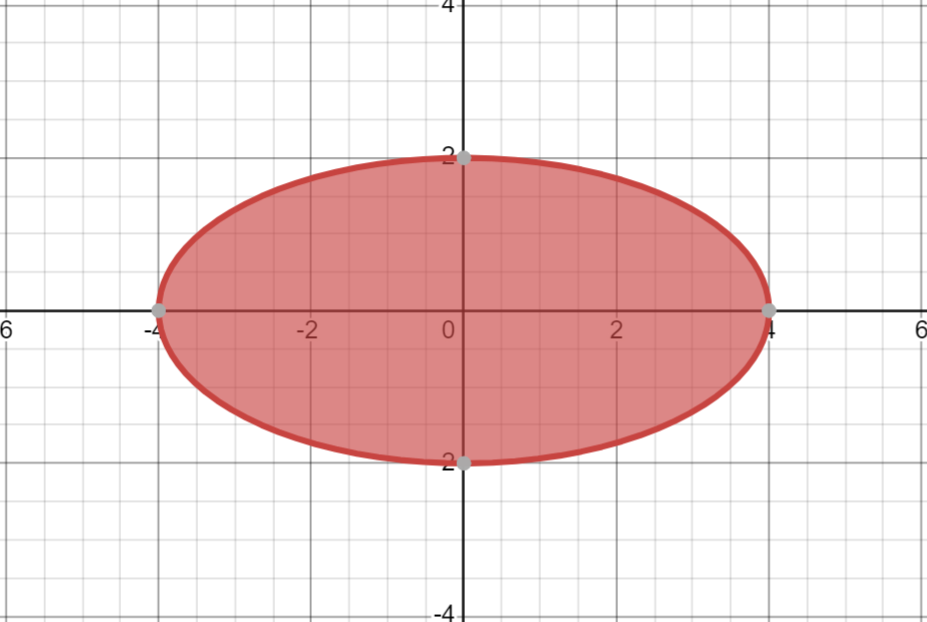
\includegraphics[width=12em]{media/1.1.png}

        $\{(x,y) \in \mathbb R^2:x^2+4y^2\leq16\}$

        \item \phantom{ }
        
        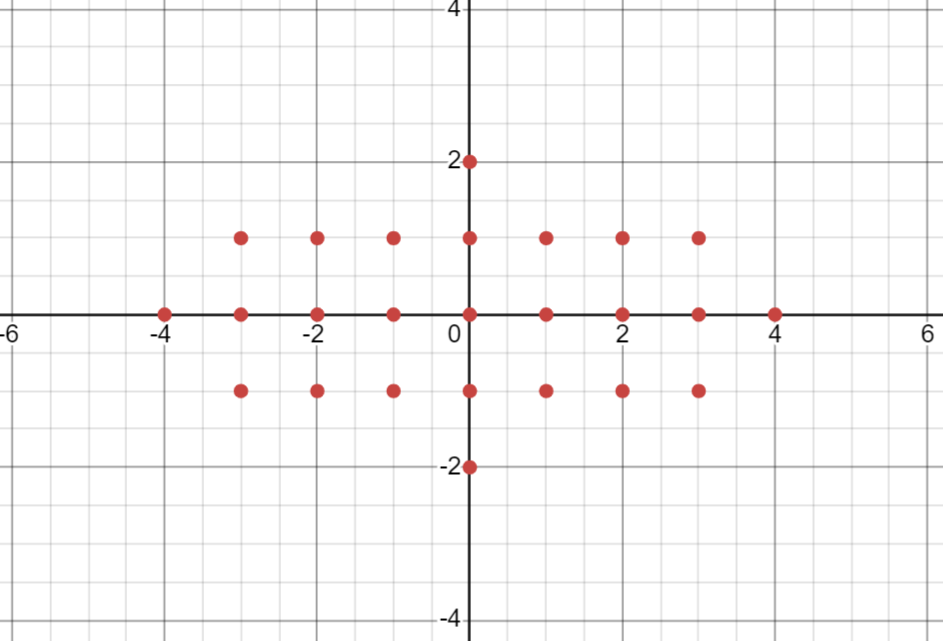
\includegraphics[width=12em]{media/1.2.png}

        $\{(x,y) \in \mathbb Z^2:x^2+4y^2\leq16\}$

        \item \phantom{ }
        
        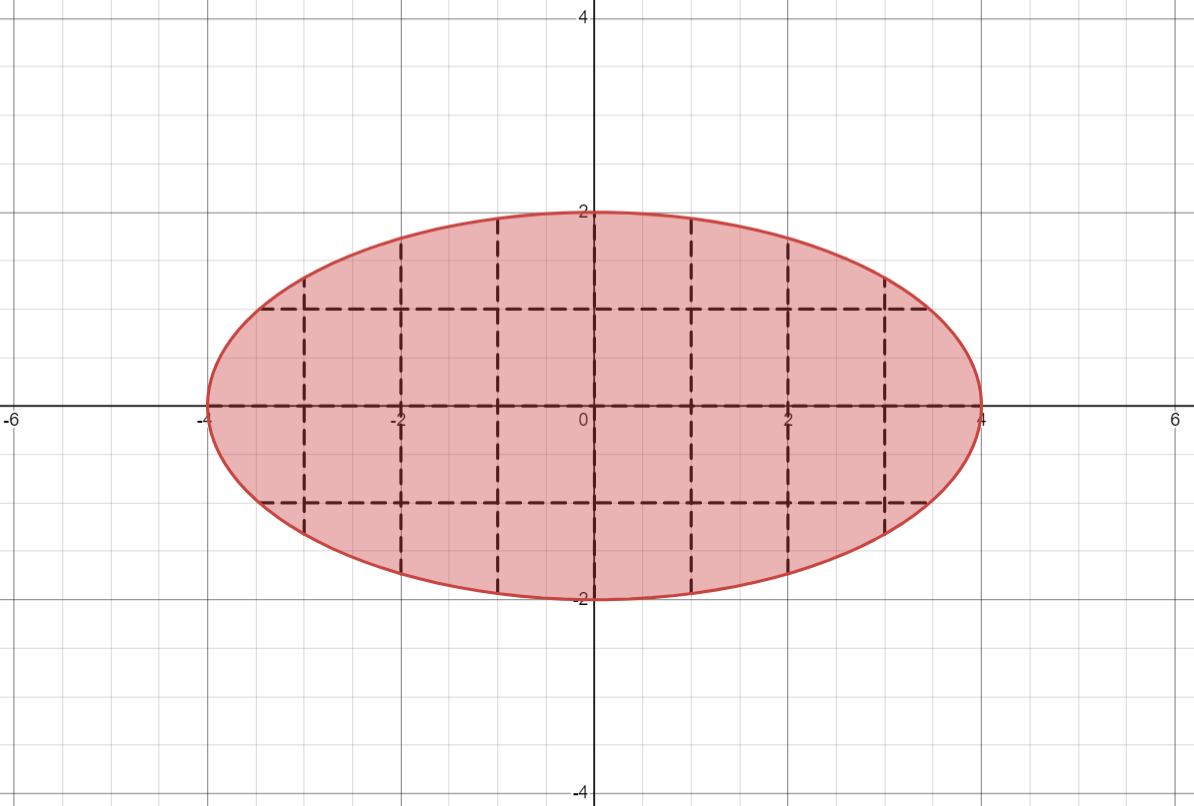
\includegraphics[width=12em]{media/1.3.png}
    \end{enumerate}
\end{soln}
%%%%%%%%%%%%%%%%%%%%%%%%%%%%%%%%%%%%%%%%%%%%%%%%%%%%%%%%%%%%%%%%%%%%%%%%%%%%%%
\begin{problem}
	Let $\Ff = \{A\subseteq\N\,:\,|A| \text{ is finite}\}$.
	Determine whether each of the following is true or false; justify your answer.
	\begin{enumerate}
		\item $\N\in\Ff$.
		\item If $A\in\Ff$, then $\overline A\in\Ff$.
		\item $|\Ff|$ is finite.
		\item If $A_1, A_2,\ldots \in\Ff$, then $\displaystyle\bigcup_{n=1}^\infty A_n\in\Ff$.
		\item If $A_1, A_2,\ldots \in\Ff$, then $\displaystyle\bigcap_{n=1}^\infty A_n\in\Ff$.
	\end{enumerate}
	
\end{problem}

\begin{soln}
	
\end{soln}

%%%%%%%%%%%%%%%%%%%%%%%%%%%%%%%%%%%%%%%%%%%%%%%%%%%%%%%%%%%%%%%%%%%%%%%%%%%%%%
\begin{problem}
	For each $\alpha\in\R$, define $A_\alpha = \{(x,\alpha\cos x)\in\R^2\,:\, -2\pi\leq x\leq 2\pi\}$.
	Describe the following sets in set-builder notation and draw them in the plane $\R^2$.
	\begin{enumerate}
		\item $\displaystyle A_\frac{1}{2}$
		\item $\displaystyle\bigcup_{\alpha\in\Z} A_\alpha$
		\item $\displaystyle\bigcap_{\alpha\in\Z} A_\alpha$
		\item $\displaystyle\bigcup_{\alpha\in\R} A_\alpha$
		\item $\displaystyle\bigcap_{\alpha\in\R} A_\alpha$
	\end{enumerate}
\end{problem}

\begin{soln}
	
\end{soln}
%%%%%%%%%%%%%%%%%%%%%%%%%%%%%%%%%%%%%%%%%%%%%%%%%%%%%%%%%%%%%%%%%%%%%%%%%%%%%%
\end{document}